% SVN in for this file
\svnidlong
{$HeadURL$}
{$LastChangedDate$}
{$LastChangedRevision$}
{$LastChangedBy$}

\chapter{Serie di potenze}
\labelChapter{seriedipotenze}

\begin{introduction}
	‘‘BEEP BOOP QUESTA È UNA CITAZIONE.''
	\begin{flushright}
		\textsc{Marinobot,} dopo aver finito le citazioni stupide.
	\end{flushright}
\end{introduction}
\lettrine[findent=1pt, nindent=0pt]{L}{e} Nel \refChapter{convergenzafunzioni} abbiamo iniziato a trattare la convergenza uniforme e puntuale di successioni di funzioni. Adesso passiamo a parlare di serie di funzioni.
\textbf{[COMPLETARE]} % TO DO: completare l'intro
\section{Serie di potenze}\label{seriedipotenze}
\begin{define}
	Una \textbf{serie di potenze}\index{serie!di potenze} è una serie di funzioni della forma
	\begin{equation}
		\sum_{n=0}^{+\infty}a_n	\left(x-x_0\right)^n
	\end{equation}
	con $a_n$ numeri reali (eventualmente dipendenti da $n$) e $x,\ x_0\in A\subseteq\realset$, dove $x_0$ è dato.
\end{define}
L'ambito naturale di studio delle serie di potenze è $\complexset$: da qui in poi considereremo la serie (con anche i suoi coefficienti) in campo complesso:
\begin{equation}
	\sum_{n=0}^{+\infty}a_n	\left(z-z_0\right)^n\qquad a_n,\ z\in\complexset
\end{equation}
dove $z\in A\subseteq\complexset$. Cambiando le variabili possiamo centrare la serie in $z_0=0$, cioè studiare la serie
\begin{equation}
	\sum_{n=0}^{+\infty}a_nz^n=a_0+a_1z+a_2z^2+a_3z^3\ldots
\end{equation}
Chiaramente la serie così scritta converge in $z=0$ (o, se prendiamo la serie \textit{non} centrata nell'origine, in $z=z_0$), dato che la serie ha termini \textit{costantemente nulli} e quindi è banalmente convergente.\\
Ci interessa ora studiare in quale insieme di $\complexset$ tali serie convergono. 
\begin{theorema}[Insieme di convergenza.]~{}\\\label{insiemediconvergenza}
	Se una serie di potenze converge in $z_0\in\complexset$, allora essa converge (assolutamente) in ogni punto $z$ con $\abs{z}<\abs{z_0}$.
\end{theorema}
\begin{demonstration}
	Sappiamo dalle ipotesi che la serie $\displaystyle\sum_{n=0}^{+\infty}a_nz_0^n$ è convergente, quindi per la condizione necessaria di convergenza il termine $a_nz_0^n$ tende a zero. Per definizione di limite significa che
	\begin{equation*}
		\forall \epsilon >0\ \exists N=N\left(\epsilon\right)\in\naturalset\colon\forall n\geq N\ \abs{a_nz_0^n}<\epsilon
	\end{equation*}
	Scegliamo arbitrariamente $\epsilon = 1$, cioè $\exists N_1=N\left(1\right)\colon \forall n\geq N$ vale $\abs{a_nz_0^n}<1$.
	Allora definitivamente vale
	\begin{equation*}
		\abs{a_nz^n}=\abs{a_nz_0^n}\abs{\frac{z}{z_0}}^n\leq\abs{\frac{z}{z_0}}^n
	\end{equation*}
	Poiché per ipotesi $\abs{z}<\abs{z_0}$, vale $\abs{\frac{z}{z_0}}<1$ e quindi la serie geometrica $\displaystyle\sum_{n=0}^{+\infty}\abs{\frac{z}{z_0}}$ converge. Per il teorema di confronto segue che anche la serie $\displaystyle\sum_{n=0}^{+\infty}\abs{a_nz^n}$ è convergente e quindi $\displaystyle\sum_{n=0}^{+\infty}a_nz^n$ converge (assolutamente).
\end{demonstration}
Con questo non solo abbiamo dimostrato che se la serie di potenze converge in $z_0$ la serie converge in tutti i punti $z$ con $\abs{z}<\abs{z_0}$, ma implicitamente sappiamo anche che la serie \textit{non} converge in $z_0$ allora \textit{non} converge per $\abs{z}>\abs{z_0}$.\\
Infatti, se in $z_0$ la serie non converge supponiamo per assurdo che esista $z^\ast$, con $\abs{z^\ast}>\abs{z_0}$, in cui la serie converge. Per il teorema appena dimostrato in tutti i punti $z$ con $\abs{z}<\abs{z^\ast}$ la serie di potenze converge, ma fra questi è compreso anche $z_0$ dove essa \textit{non} converge.
\subsection{Il raggio di convergenza}
Per queste osservazioni l'insieme di convergenza della serie è un \textit{cerchio} centrato nell'origine di un certo \textit{raggio} $R$. Diamo una definizione formale di questo raggio.
\begin{define}[Cerchio e raggio di convergenza.]~{}\\
	Preso $\displaystyle A=\left\{z\middle\vert\sum_{n=0}^{+\infty} a_n z^n \ \mbox{converge} \right\}\subseteq \complexset$ l'insieme di convergenza della serie di potenze centrata in $z_0=0$ e consideriamo l'insieme $E=\left\{\abs{z}\mid z\in A\right\}\subseteq\realset$ dato da tutti i moduli dei punti di convergenza della serie. Il \textbf{raggio di convergenza}\index{raggio di convergenza} è definito come
	\begin{equation*}
		r\coloneqq\sup E=\sup\left\{\abs{z}\middle\vert\sum_{n=0}^{+\infty} a_n z^n \ \mbox{converge} \right\}
	\end{equation*}
	Esso può essere:
	\begin{itemize}
		\item $R=0$; in tal caso la serie converge \textit{solo} per $z=0$.
		\item $R=+\infty$; in tal caso la serie converge \textit{per ogni} $z\in\complexset$.
		\item $0<R<+\infty$; in base al teorema \ref{insiemediconvergenza}, pag. \ref{insiemediconvergenza}, la serie converge (assolutamente) per $\abs{z}<r$, \textit{non} converge per $\abs{z}<r$ e a priori non abbiamo \textit{alcuna informazione} per i punti $z$ sul \textit{bordo}, cioè tali che $\abs{z}=r$. L'\textit{insieme di convergenza} risulta essere un \textbf{cerchio aperto}\index{cerchio di convergenza} centrato nell'origine di raggio $R$, a cui si aggiungono eventualmente altri punti di convergenza sul \textit{bordo} (tutti, nessuno o solo alcuni).
	\end{itemize}
	\begin{center}
		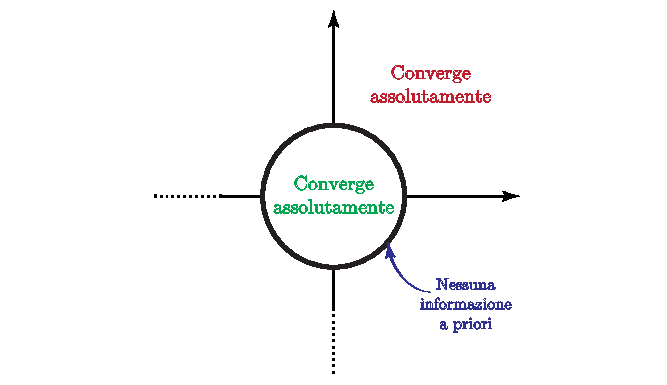
\includegraphics[trim=2.5cm 0.5cm 2.5cm 0cm, clip, scale=1]{images/discoconvergenza.pdf}
	\end{center}
\end{define}
Poiché sappiamo che la serie converge assolutamente per $\abs{z}<r$, lo studio del raggio di convergenza passa attraverso lo studio della serie assoluta associata $\displaystyle\sum_{n=0}^{+\infty}\abs{a_nz^n}$.\\
Per determinare il raggio di convergenza, possiamo ad esempio usare la \textbf{legge di D’Alembert}\seeonlyindex{criterio!del rapporto}{legge!di D’Alembert} o detto anche \textit{criterio del rapporto}\index{criterio!del rapporto}, che ci fornisce una condizione \textit{sufficiente} su come determinare il raggio di convergenza.
\begin{proposition}[Legge di D’Alembert o criterio del rapporto.]~{}\\
	Data la serie $\displaystyle\sum_{n=0}^{+\infty}a_nz^n$, se $a_n\neq 0$ definitivamente ed esiste il limite
	\begin{equation*}
		\lim_{n\to+\infty}\frac{\abs{a_{n+1}}}{\abs{a_{n}}}=L
	\end{equation*}
	allora
	\begin{enumerate}
		\item $L=0\implies R=+\infty$
		\item $L=+\infty\implies R=0$
		\item $0<L<+\infty\implies R=\frac{1}{L}$
	\end{enumerate}
\end{proposition}
Questa proposizione ha il vantaggio di essere operativamente utile, ma ovviamente solo se valgono le ipotesi: non è scontato che il limite del rapporto sia ben definito!\\
Un teorema più generale che vale \textit{per ogni serie} è il \textit{criterio della radice}\index{criterio!della radice} o altresì noto come \textbf{legge di Cauchy-Hadamard}\seeonlyindex{criterio!del rapporto}{legge!di Cauchy-Hadamard}.
\begin{theorema}
	Sia data la serie di potenze
	\begin{equation*}
		\sum_{n=0}^{+\infty}a_nz^n
	\end{equation*}
	e sia
	\begin{equation}
		\lambda=\limsup_{n\to+\infty}\sqrt[n]{\abs{n}}
	\end{equation}
	Allora
	\begin{enumerate}
		\item Se $\lambda = 0$, la serie converge $\forall z\in\complexset$.
		\item Se $0<\lambda<+\infty$, la serie converge $R=\frac{1}{\lambda}$.
		\item Se $\lambda = +\infty$, la serie converge solo in $z=0$.
	\end{enumerate}
\end{theorema}
\begin{observe}
	I tre casi scritti esauriscono \textit{tutti} i casi possibili. Infatti, per la permanenza del segno del limsup\footnote{Nelle ‘‘Note aggiuntive'', a pagina XXX è possibile trovare la dimostrazione di questo risultato insieme ad altri relativi al limsup e liminf.} vale
	\begin{equation*}
		\sqrt[n]{\abs{a_n}}\geq 0,\ \forall n\geq 0\implies\limsup_{n\to+\infty}\sqrt[n]{\abs{a_n}}\geq 0
	\end{equation*}
\end{observe}
\begin{demonstration}\textsc{(della legge di Cauchy-Hadamard.)}~{}\\
	Partiamo dal dimostrare il punto $2)$: dobbiamo provare che $R=\frac{1}{\lambda}$, ossia
	\begin{itemize}
		\item Se $\abs{z}<\nicefrac{1}{\lambda}$, allora $\displaystyle\sum_{n=0}^{+\infty}a_nz^n$ converge.
		\item Se $\abs{z}>\nicefrac{1}{\lambda}$, allora $\displaystyle\sum_{n=0}^{+\infty}a_nz^n$ \textit{non} converge.
	\end{itemize}
	\begin{itemize}
		\item Sia $z$ tale che $\abs{z}<\nicefrac{1}{\lambda}$. Se $z=0$ la serie banalmente converge.\\
		Se $z\neq 0$, vale $\lambda<\nicefrac{1}{\abs{z}}$; consideriamo allora $\lambda'$ tale che $\lambda<\lambda'<\nicefrac{1}{\abs{z}}$: poiché $\lambda'>\lambda$, per la caratterizzazione del massimo limite si ha
		\begin{equation*}
			\textcolor{red}{\circled{\ast}}\quad\exists N\colon\forall n\geq N\ \sqrt[n]{\abs{a_n}}<\lambda'
		\end{equation*}
		Proviamo che $\displaystyle\sum_{n=0}^{+\infty}a_nz^n$ converge assolutamente usando il criterio del confronto.
		\begin{equation*}
			\abs{a_nz^n}=\abs{a_n}\abs{z^n}=\abs{a_n}\abs{z}^n\substack{<}_{\textcolor{red}{\circled{\ast}}}<\left(\lambda'\right)^n\abs{z}^n=\left(\lambda'\abs{z}\right)^n,\ \forall n\geq N
		\end{equation*}
		Questo è il termine $n$-esimo della serie geometrica $\displaystyle\sum_{n=0}^{+\infty}\left(\lambda'\abs{z}\right)^n$ di ragione $\lambda'\abs{z}$.\\
		Poiché $0<\lambda'\abs{z}<1$ per la scelta di $\lambda'$, la serie geometrica converge e quindi per il criterio del confronto converge anche la serie $\displaystyle\sum_{n=0}^{+\infty}\abs{a_nz^n}$ e dunque converge anche $\displaystyle\sum_{n=0}^{+\infty}a_nz^n$.
		\item Sia $z$ tale che $\abs{z}>\nicefrac{1}{\lambda}$. Per mostrare la non convergenza della serie proviamo che la condizione necessaria di convergenza non è soddisfatta, ovvero
		\begin{equation*}
			\lim_{n\to+\infty}a_nz^n\neq 0,\ \forall z\colon \abs{z}>\frac{1}{\lambda}
		\end{equation*}
		Questo è equivalente a mostrare che
		\begin{equation*}
			\lim_{n\to+\infty}\abs{a_nz^n}\neq 0,\ \forall z\colon \abs{z}>\frac{1}{\lambda}
		\end{equation*}
		Poiché $z\neq 0$, vale $\lambda>\nicefrac{1}{\abs{z}}$.	Consideriamo allora $\lambda''$ tale che $\nicefrac{1}{\abs{z}}<\lambda''<\lambda$: poiché $\lambda''<\lambda$, per la caratterizzazione del massimo limite si ha
		\begin{equation*}
			\textcolor{blue}{\circled{\ast}}\quad\exists n_k\to+\infty\colon\sqrt[n_k]{\abs{a_{n_k}}}>\lambda''
		\end{equation*}
		Si ha, lungo la sottosuccessione:
		\begin{equation*}
			\abs{a_{n_k}z^{n_k}}=\abs{a_n}{z}^{n_k}\substack{>}_{\textcolor{blue}{\circled{\ast}}}>\left(\lambda''\right)^{n_k}\abs{z}^{n_k}=\left(\substack{\lambda''\abs{z}}_{>1\text{ per la scelta di }\lambda''}\right)^{n_k}>1,\ \forall n_k
		\end{equation*}
		Poiché esiste una sottosuccessione che è sempre maggiore di $1$, deve esistere un valore limite della successione $\abs{a_nz^n}$ maggiore o uguale a $1$. Ma allora
		\begin{equation*}
			\limsup_{n\to+\infty}\abs{a_nz^n}\geq 1\implies\lim_{n\to+\infty}\abs{a_nz^n}\neq 0
		\end{equation*}
	\end{itemize}
	La dimostrazione del punto $1)$ è analoga alla prima parte della dimostrazione del punto $2)$. In questo caso, dobbiamo mostrare che la serie converge $\forall z\in\complexset$.\\ Se $z=0$, la serie banalmente converge, mentre se $z\neq 0$, si ha chiaramente che $0=\lambda<\nicefrac{1}{\abs{z}},\ \forall z\in\complexset\setminus\{0\}$. Consideriamo allora $\lambda'$ tale che $0<\lambda'<\nicefrac{1}{\abs{z}}$: poiché $\lambda'>0$, per la caratterizzazione del massimo limite si ha
	\begin{equation*}
		\textcolor{red}{\circled{\ast}}\quad\exists N\colon\forall n\geq N\ \sqrt[n]{\abs{a_n}}<\lambda'
	\end{equation*}
	Proviamo che $\displaystyle\sum_{n=0}^{+\infty}a_nz^n$ converge assolutamente usando il criterio del confronto.
	\begin{equation*}
		\abs{a_nz^n}=\abs{a_n}\abs{z^n}=\abs{a_n}\abs{z}^n\substack{<}_{\textcolor{red}{\circled{\ast}}}<\left(\lambda'\right)^n\abs{z}^n=\left(\lambda'\abs{z}\right)^n,\ \forall n\geq N
	\end{equation*}
	Questo è il termine $n$-esimo della serie geometrica $\displaystyle\sum_{n=0}^{+\infty}\left(\lambda'\abs{z}\right)^n$ di ragione $\lambda'\abs{z}$.\\
	Poiché $0<\lambda'\abs{z}<1$ per la scelta di $\lambda'$, la serie geometrica converge e quindi per il criterio del confronto converge anche la serie $\displaystyle\sum_{n=0}^{+\infty}\abs{a_nz^n}$ e dunque converge anche $\displaystyle\sum_{n=0}^{+\infty}a_nz^n$. Poiché la scelta di $z$ è stata arbitraria, vale la tesi.\\
	La dimostrazione del punto $1)$ è analoga alla seconda parte della dimostrazione del punto $2)$. In questo caso, dobbiamo mostrare che la serie converge solo in $z=0$.\\ Se $z=0$, la serie banalmente converge. Per mostrare la non convergenza della serie proviamo che la condizione necessaria di convergenza non è soddisfatta, ovvero
	\begin{equation*}
		\lim_{n\to+\infty}a_nz^n\neq 0,\ \forall z\neq 0
	\end{equation*}
	Questo è equivalente a mostrare che
	\begin{equation*}
		\lim_{n\to+\infty}\abs{a_nz^n}\neq 0,\ \forall z\neq 0
	\end{equation*}
	Dato $z\neq 0$, consideriamo allora $\lambda''$ tale che $\nicefrac{1}{\abs{z}}<\lambda''<+\infty$: poiché $\lambda''<+\infty$, per la caratterizzazione del massimo limite si ha
	\begin{equation*}
		\textcolor{blue}{\circled{\ast}}\quad\exists n_k\to+\infty\colon\sqrt[n_k]{\abs{a_{n_k}}}>\lambda''
	\end{equation*}
	Si ha, lungo la sottosuccessione:
	\begin{equation*}
		\abs{a_{n_k}z^{n_k}}=\abs{a_n}{z}^{n_k}\substack{>}_{\textcolor{blue}{\circled{\ast}}}>\left(\lambda''\right)^{n_k}\abs{z}^{n_k}=\left(\substack{\lambda''\abs{z}}_{>1\text{ per la scelta di }\lambda''}\right)^{n_k}>1,\ \forall n_k
	\end{equation*}
	Poiché esiste una sottosuccessione che è sempre maggiore di $1$, deve esistere un valore limite della successione $\abs{a_nz^n}$ maggiore o uguale a $1$. Ma allora
	\begin{equation*}
		\limsup_{n\to+\infty}\abs{a_nz^n}\geq 1\implies\lim_{n\to+\infty}\abs{a_nz^n}\neq 0
	\end{equation*}
	La scelta di $z$ è arbitraria, purché $z$ sia diverso da zero; per questo motivo vale la tesi.
\end{demonstration}
\section{Comportamento sul bordo}
Consideriamo la serie di potenze
\begin{equation*}
	\sum_{n=0}^{+\infty}a_nz^n,\quad a_n,\ z\in\complexset
\end{equation*}
con raggio di convergenza finito e non nullo.
I possibili comportamenti sul \textit{bordo} del cerchio di convergenza sono i seguenti:
\begin{enumerate}
	\item Convergenza in \textit{tutti i punti} del bordo del cerchio di convergenza
	\item \textit{Non} convergenza in \textit{nessun punto} del bordo del cerchio di convergenza
	\item Convergenza solo in \textit{alcuni punti} del bordo del cerchio di convergenza
\end{enumerate}
Mostriamo per ciascuno di essi un esempio.
\begin{example}\textsc{Caso 1.}~{}\\
	Consideriamo la serie
	\begin{equation*}
		\sum_{n=1}^{+\infty}\frac{z^n}{n^\alpha},\quad\alpha>1
	\end{equation*}
	Con la formula di D'Alembert vediamo che il raggio di convergenza è $R=1$. Infatti
	\begin{equation*}
		\lim_{n\to+\infty}\frac{\abs{a_{n+1}}}{\abs{a_{n}}}=\lim_{n\to+\infty}\frac{\left(n+1\right)^\alpha}{n^\alpha}=\lim_{n\to+\infty}\frac{n^\alpha\left(1+\frac{1}{n}\right)^\alpha}{n^\alpha}=\lim_{n\to+\infty}\left(1+\frac{1}{n}\right)^\alpha=1=\mathcal{l}\implies r=\frac{1}{\mathcal{l}}=1
	\end{equation*}
	Per ogni $z\in\complexset$ tale che $\abs{z}=1$ la serie converge (assolutamente):
	\begin{equation*}
		\sum_{n=1}^{+\infty}\abs{\frac{z^n}{n^\alpha}}=\sum_{n=1}^{+\infty}\frac{n}{n^\alpha}
	\end{equation*}
	La serie in modulo è la \textit{serie armonica generalizzata} che, per $\alpha>1$, converge; la serie semplice converge su tutti i punti del bordo.
\end{example}
\begin{example}\textsc{Caso 2.}~{}\\
	Consideriamo la \textit{serie geometrica}
	\begin{equation*}
		\sum_{n=1}^{+\infty}z^n
	\end{equation*}
	Poichè $a_n\equiv 1\ \forall n$, il criterio del rapporto ci fornisce come raggio di convergenza $R=1$.\\
	Per ogni $z\in\complexset$ tale che $\abs{z}=1$ la serie \textit{non} converge: possiamo osservare che presa la successione $c_n\in\complexset$, vale\footnote{Nelle ‘‘Note aggiuntive'', a pagina XXX è possibile trovare la dimostrazione di questo risultato.}
	\begin{equation*}
		\lim_{n\to+\infty}\abs{c_n}\neq 0\implies\lim_{n\to+\infty}c_n\neq 0
	\end{equation*}
	In questo caso:
	\begin{equation*}
		\lim_{n\to+\infty}\abs{z^n}=\lim_{n\to+\infty}1=1\neq 0\implies\lim_{n\to+\infty}z^n\neq 0
	\end{equation*}
	È evidente che la \textit{condizione necessaria} di convergenza \textit{non} è soddisfatta: la serie \textit{non} converge in nessun punto del bordo.
\end{example}
\begin{example}\textsc{Caso 3.}~{}\\
	Consideriamo la serie
	\begin{equation*}
		\sum_{n=1}^{+\infty}\frac{z^n}{n^\alpha},\quad0<\alpha<1
	\end{equation*}
	L'applicazione del criterio del confronto è esattamente analogo a quello visto nel caso  e il raggio di convergenza è pertanto $R=1$.\\
	Se $z=1$ la serie \textit{non} converge, dato che essa diventa una serie armonica generalizzata con $\alpha\leq1$:
	\begin{equation*}
		\sum_{n=1}^{+\infty}\frac{1}{n^\alpha}
	\end{equation*}
	Invece, per ogni $z\in\complexset$ tale che $\abs{z}=1$ e $z\neq 1$ la serie converge: infatti, possiamo applicare il \textit{criterio di Abel-Dirichlet}.
	\begin{equation*}
		\sum_{n=1}^{+\infty}\frac{z^n}{n^\alpha}=\sum_{n=1}^{+\infty}z^n\frac{1}{n^\alpha}=\sum_{n=1}^{+\infty}\alpha_n\beta_n
	\end{equation*}
	con $\alpha_n=z^n$ e $\beta_n=\nicefrac{1}{n^\alpha},\ n\geq 1$.
	\begin{enumerate}
		\item $\beta_n=\nicefrac{1}{n^\alpha}$ è una successione di elementi strettamente positivi, decrescenti e infinitesima per $n\to+\infty$.
		\item La successione delle \textit{somme parziali} di $\alpha_n=z^n$ è \textit{limitata}. Consideriamo
		\begin{equation*}
			\abs{\sum_{n=1}^{k}z^n}=\abs{\sum_{n=0}^{k}z^n-1}\squarequal
		\end{equation*}
		Poiché $\displaystyle\sum_{n=0}^{k}z^n$ è un serie geometrica parziale, sappiamo la sua somma parziale. Applicando poi una \textit{disuguaglianza triangolare}, troviamo una \textit{maggiorazione} della somma parziale di $\alpha_n$.
		\begin{equation*}
			\squarequal\abs{\frac{1-z^{k+1}}{1-z}-1}=\abs{\frac{z-z^{k+1}}{1-z}}\leq\frac{\abs{z}+\abs{-z^{k+1}}}{\abs{1-z}}\leq\frac{1+1}{\abs{1-z}}=\frac{2}{\abs{1-z}},\ \forall k\geq 1
		\end{equation*}
	\end{enumerate}
	Osserviamo che, nonostante la serie converga, essa non converge assolutamente: la serie in modulo è la serie armonica generalizzata con $\alpha\leq 1$, nota per essere divergente.
\end{example}
Anche se in generale non possiamo affermare a priori come converge sul bordo si può osservare che, in alcuni casi particolari, dalla converge in un punto del bordo si ottiene la convergenza sull'intero bordo. Vediamone alcuni
\begin{proposition}[Convergenza assoluta sul bordo se la serie di potenze converge assolutamente in un punto.]~{}\\
	Sia data la serie di potenze
	\begin{equation*}
		\sum_{n=1}^{+\infty}a_nz^n
	\end{equation*}
	Se la serie converge assolutamente in un punto della frontiera del cerchio di convergenza, allora converge assolutamente su tutta questa frontiera.
\end{proposition}
\begin{demonstration}
	Supponiamo che la serie converga assolutamente in $z_0$, dove $\abs{z_0}=R$ e prendiamo un qualunque $z$ tale che $\abs{z}=R$.
	Osserviamo che, presa la serie in modulo, si ha
	\begin{equation*}
		\sum_{n=1}^{+\infty}\abs{a_nz^n}=\sum_{n=1}^{+\infty}\abs{a_n}\abs{z^n}=\sum_{n=1}^{+\infty}\abs{a_n}\abs{z}^n=\sum_{n=1}^{+\infty}\abs{a_n}R^n=\sum_{n=1}^{+\infty}\abs{a_n}ì\abs{z_0}^n=\sum_{n=1}^{+\infty}\abs{a_nz_0^n}
	\end{equation*}
	che converge per ipotesi. Allora la serie di potenze converge assolutamente.
\end{demonstration}
\begin{corollary}[Convergenza sul bordo se la serie di potenze a coefficienti reali positivi converge in $z=R$.]~{}\\
	Sia data la serie di potenze
	\begin{equation*}
		\sum_{n=1}^{+\infty}a_nz^n
	\end{equation*}
	Se la serie ha coefficienti reali positivi e converge nel punto $z=R$, dove $R\in\left(0,+\infty\right)$ è il raggio di convergenza, allora converge in ogni punto della frontiera del cerchio di convergenza.
\end{corollary}
\begin{demonstration}
	Poiché $a_n$ e $R$ sono reali positivi, $a_n=\abs{a_n}$ e $R=\abs{R}$. Allora si ha
	\begin{equation*}
		\sum_{n=1}^{+\infty}a_nR^n=\sum_{n=1}^{+\infty}\abs{a_nR^n}
	\end{equation*}
	Quindi in questo caso la convergenza semplice della serie implica la convergenza assoluta. Poiché la serie converge assolutamente in un punto del bordo, segue dalla proposizione precedente la convergenza (assoluta) in tutti i punti del bordo.
\end{demonstration}
\section{Serie di potenze e convergenza uniforme}
\begin{theorema}[Converge uniforme delle serie di potenze.]~{}\\\label{convergenzasottoinsiemeH}
	Sia $\displaystyle\sum_{n=0}^{+\infty}a_nz^n$ una serie di potenze con raggio di convergenza $R\in\left(0,+\infty\right)$. Allora
	\begin{enumerate}
		\item La serie converge uniformemente su ogni insieme $H\subseteq\complexset$ tale che $\overline{H}\subsetneqq B_R\left(0\right)$, con $B_R\left(0\right)$ il disco aperto di convergenza.
		\item Se la serie converge assolutamente in ogni $z\in\partial B_R\left(0\right)$ (il bordo del disco), allora converge uniformemente sul disco chiuso $\overline{B_R\left(0\right)}$.
	\end{enumerate}
\end{theorema}
\begin{demonstration} Per questa dimostrazione useremo il \textit{criterio di Weierstrass} enunciato nella sezione \ref{criteriodiweierstrass}, pag. \pageref{criteriodiweierstrass}.
	\begin{enumerate}
		\item Sia $H$ tale che $\overline{H}\subsetneqq B_R\left(0\right)$. Per il criterio di Weierstrass, per provare la convergenza uniforme su $H$ è sufficiente provare che esiste una successione $c_n$ tale che
		\begin{enumerate}
			\item $\abs{a_nz^n}\leq c_n,\ \forall z\in H$
			\item $\displaystyle\sum_{n=0}^{+\infty}c_n$ converge.
		\end{enumerate}
		\begin{minipage}{0.40\textwidth}
			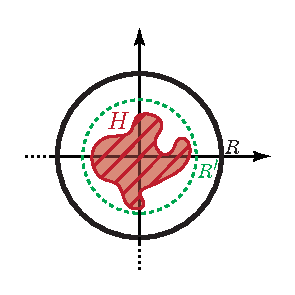
\includegraphics[trim=0cm 0cm 0cm 0cm, clip, scale=1]{images/discoconvergenzainsiemeH.pdf}
		\end{minipage}\hspace{-7mm}
		\begin{minipage}{0.55\textwidth}
			Poiché $H$ è solo \textit{strettamente contenuto} nel disco aperto di convergenza, $\exists R'<R$ tale che si abbia $\overline{H}\subseteq B_{R'}\left(0\right)$, ossia $\abs{z}\leq R',\ \forall z\in H$.\\
			Allora si ha, $\forall n\geq 0$ e $\forall z\in H$
			\begin{equation*}
				\abs{a_nz^n}=\abs{a_n}\abs{z}^n\leq \underbrace{\abs{a_n}\left(R'\right)^n}_{\text{non dipende da }z}
			\end{equation*}
		\end{minipage}\\
		Inoltre, la serie $\displaystyle\sum_{n=0}^{+\infty}c_n=\sum_{n=0}^{+\infty}\abs{a_n}\left(R'\right)^n$ converge in quanto è la convergenza della serie di potenze per il punto $z=R'$, che è \textit{interno} al disco di convergenza $B_R\left(0\right)$. Applicando il criterio di Weierstrass otteniamo la tesi.
		\item Si ripete la dimostrazione sull'insieme $\overline{B_R\left(0\right)}$ con $R'=R$, considerando che la serie $\displaystyle\sum_{n=0}^{+\infty}\abs{a_n}R^n$ converge per ipotesi sulla convergenza sul bordo.
	\end{enumerate}
\end{demonstration}
\begin{example}\textsc{Serie geometrica.}\\
	Sulla \textit{serie geometrica} $\displaystyle\sum_{n=0}^{+\infty}z^n$ abbiamo già ricavato diverse informazioni: ha raggio di convergenza $R=1$ e \textit{non} c'è convergenza (assoluta) sul bordo. Studiamo ora la convergenza uniforme.
	\begin{itemize}
		\item Converge uniformemente su ogni insieme $H$ tale che $\overline{H}\subsetneqq B_1\left(0\right)$ per il teorema precedente.
		\item Non avendo alcuna convergenza sul bordo, a priori non possiamo dare risultati generali sulla convergenza uniforme sulla base del teorema visto. Tuttavia, possiamo mostrare direttamente - grazie al fatto che la somma parziale e limite della serie geometrica è nota\footnote{Nelle ‘‘Note aggiuntive'', a pagina XXX è possibile trovare maggiori dettagli sulla somma (parziale) della serie geometrica e come ricavarla.} -  che la serie non converge uniformemente sul disco aperto $B_1\left(0\right)$. Infatti
		\begin{align*}
			\sup_{z\in B_1\left(0\right)}\abs{S_n\left(z\right)-S\left(z\right)}&=\sup_{z\in B_1\left(0\right)}\abs{\frac{1-z^{n+1}}{1-z}-\frac{1}{1-z}}=\sup_{z\in B_1\left(0\right)}\abs{\frac{-z^{n+1}}{1-z}}=\\
			&=\sup_{z\in B_1\left(0\right)}\frac{\abs{z}^{n+1}}{\abs{1-z}}=+\infty,\ \forall n\geq 0
		\end{align*}
		da cui
		\begin{equation*}
			\lim_{n\to+\infty}\left(\sup_{z\in B_1\left(0\right)}\abs{S_n\left(z\right)-S\left(z\right)}\right)=+\infty\neq 0
		\end{equation*}
	\end{itemize}
\end{example}
\section{Proprietà di regolarità della somma di una serie di potenze}
Sia $\displaystyle\sum_{n=0}^{+\infty}a_nz^n$ una serie di potenze con $R>0$ il raggio di convergenza. Studiamo le proprietà di continuità e derivabilità della \textbf{funzione somma}\index{funzione!somma}
\begin{equation}
	\funztot{f}{B_R\left(0\right)\subseteq\complexset}{\complexset}{z}{\displaystyle\sum_{n=0}^{+\infty}a_nz^n}
\end{equation}
\subsection{Continuità}
\begin{proposition}[Proprietà di continuità per la somma di una serie di potenze, caso generale.]~{}\\
	La funzione $f$ è continua su $B_R\left(0\right)$.
\end{proposition}
\begin{attention}
	La convergenza della serie di potenze su $B_R\left(0\right)$ \textit{non} è in generale uniforme, ma sappiamo al più che converge uniformemente su $H$ tale che $\overline{H}\subsetneqq B_R\left(0\right)$, quindi dobbiamo tenere conto di questo fattore nelle dimostrazioni che faremo.
\end{attention}
\begin{demonstration}
	Dobbiamo provare che $f\in\mathcal{C}\left(B_R\left(0\right)\right)$, cioè $f$ continua in $z_0,\ \forall z_0\in B_R\left(0\right)$.	\vspace{3mm}
	\begin{minipage}{0.44\textwidth}
		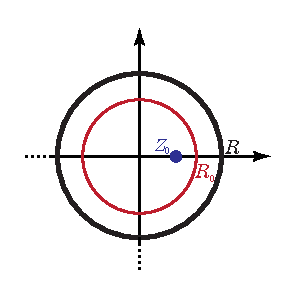
\includegraphics[trim=0cm 0cm 0cm 0cm, clip, scale=1.1]{images/discoconvergenzacontinuitaf.pdf}
	\end{minipage}\hspace{-9mm}
	\begin{minipage}{0.60\textwidth}
		Sia $z_0\in B_R\left(0\right)$ fissato. Per proprietà della metrica, allora $\exists R_0 < R$ tale che $z_0\in B_{R_0}\left(0\right)$. Su $B_{R_0}\left(0\right)$ si ha continuità uniforme e dunque, posto
		\begin{equation*}
			S_n\left(z\right)=\sum_{k=0}^{n}a_kz^k
		\end{equation*}
		si ha
		\begin{enumerate}
			\item $S_n$ continua su $B_{R_0}\left(0\right)$ perché è un polinomio.
			\item $S_n$ converge uniformemente a $f$ su $B_R\left(0\right)$.
		\end{enumerate}
	\end{minipage}\\
	Per il teorema di continuità della funzione limite, $f$ è continua in $B_{R_0}\left(0\right)$ e dunque in $z_0$. 
\end{demonstration}
Questo risultato ci permette di parlare della convergenza sul disco aperto, ma se c'è qualche tipo di convergenza sul bordo, e quindi $f$ è definita anche su di esso, si può estendere la continuità di $f$ fino a tale frontiera? Studiamo due casi.
\begin{corollary}[Proprietà di continuità per la somma di una serie di potenze, caso sul bordo con convergenza assoluta.]~{}\\
	Sia data la serie di potenze $\displaystyle\sum_{n=0}^{+\infty}a_nz^n$ con raggio di convergenza $R>0$. Se la serie converge (assolutamente) su $\partial B_R\left(0\right)$ allora la serie è continua su $\overline{B_R\left(0\right)}$.
\end{corollary}
\begin{demonstration}
	Segue immediatamente ricordando che dalle ipotesi di convergenza assoluta sul bordo, sulla base del teorema \ref{convergenzasottoinsiemeH}, pag. \pageref{convergenzasottoinsiemeH}, vale la convergenza uniforme su $\overline{B_R\left(0\right)}$.
\end{demonstration}
Se invece supponiamo che la serie converga in un punto\footnote{Nel caso di più punti di convergenza $z_0,\ z_1,\ \ldots$, la funzione somma $f$ sarà definita su $B_R\left(0\right)\cup\left\{z_0\right\}\cup\left\{z_1\right\}\cup\ldots$. Qui riportiamo per semplicità il caso di un solo punto, ma i risultati successivi sono opportunamente generalizzabili con più punti di convergenza sul bordo.} $z_0$, cioè $\displaystyle\sum_{n=0}^{+\infty}a_nz_0^n$ converge, possiamo definire la \textbf{funzione somma}\index{funzione!somma} come
\begin{equation}
	\funztot{f}{B_R\left(0\right)\cup\left\{z_0\right\}\subseteq\complexset}{\complexset}{z}{\displaystyle\sum_{n=0}^{+\infty}a_nz^n}
\end{equation}
La convergenza uniforme di $f$ anche sui punti di convergenza $z_0$ sul bordo ci viene garantita dal \textbf{teorema di Abel}\index{teorema!di Abel}.
\begin{theorema}[Teorema di Abel.]~{}\\
	Sia dato la serie di potenze la serie di potenze $\displaystyle\sum_{n=0}^{+\infty}a_nz^n$ con raggio di convergenza $R>0$. Se $\exists z_0=Re^{i\theta_0}$ tale che $\displaystyle\sum_{n=0}^{+\infty}a_nz_0^n$ converge, allora\\
	\begin{minipage}{0.39\textwidth}
		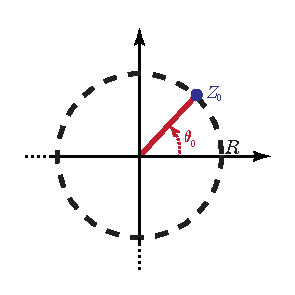
\includegraphics[trim=0cm 0cm 0cm 0cm, clip, scale=1]{images/discoconvergenzaabel.pdf}
	\end{minipage}\hspace{-12mm}
	\begin{minipage}{0.65\textwidth}
		\begin{enumerate}
			\item la serie converge uniformemente sul \textit{segmento}
			\begin{equation}
				\Sigma_0=\left\{z\in\complexset\mid z=re^{i\theta_0},\ r\in\left[0,R\right]\right\}
			\end{equation}
			\item La restrizione di $f$ a $\Sigma_0$ è \textit{continua} su $z_0$, ossia
			\begin{equation}
				\lim_{r\to R}f\left(re^{i\theta_0}\right)=f\left(z_0\right)=\sum_{n=0}^{+\infty}a_nz_0^n
			\end{equation}
		\end{enumerate}
	\end{minipage}
\end{theorema}
\subsection{Derivabilità}
Abbiamo definito la funzione somma dal disco aperto $B_R\left(0\right)$ in campo complesso a $\complexset$, ma al momento non conosciamo cosa vuol dire derivabilità di una funzione $\funz{f}{\complexset}{\complexset}$. Per il momento, limitiamoci al caso reale, cioè consideriamo una serie di potenze
\begin{equation*}
	\sum_{n=0}^{+\infty}a_nx^n,\ x\in\realset,\ a_n\in\realset
\end{equation*}
con raggio di convergenza $R>0$. In questo caso il cerchio di convergenza è un intervallo $\left(-R,R\right)$, con estremi eventualmente inclusi. La funzione somma risulta allora la funzione
\begin{equation}
	\funztot{f}{\left(-R,R\right)}{\realset}{x}{\sum_{n=0}^{+\infty}a_nx^n}
\end{equation}
\begin{theorema}[Derivabilità della somma di una serie di potenze.]~{}\\
	Sia data
	\begin{equation*}
		f\left(x\right)=\sum_{n=0}^{+\infty}a_nx^n,\ \forall x\in\left(-R,R\right),\ a_n\in\realset
	\end{equation*}
con $R>0$ il raggio di convergenza. Allora
\begin{enumerate}
	\item $f$ è derivabile su $\left(-R,R\right)$
	\item La derivata di $f$ è
	\begin{equation}
		f'\left(x\right)=\sum_{n=1}^{+\infty}na_nx^{n-1},\ \forall x\in\left(-R,R\right)
	\end{equation}
\end{enumerate}
\end{theorema}
Per dimostrare questo teorema useremo il teorema di derivibilità per serie di funzioni (teorema \ref{derivabilitatermineatermine}, pag. \pageref{derivabilitatermineatermine}, capitolo \refChapter{seriefunzioni}): poiché le ipotesi $1)$ e $2)$ sono banalmente verificate, dobbiamo contrarci sull'ipotesi $3)$, ovvero abbiamo bisogno di informazioni sulla convergenza uniforme della serie delle derivate $\displaystyle\sum_{n=1}^{+\infty}na_nx^{n-1}$; poiché la serie delle derivate è ancora una serie di potenze, allora ci basta studiare il raggio di convergenza.
% TO DO: nelle Note extra a pagina XXX inserire il prodotto del lim sup
\begin{lemming}[Convergenza della serie di derivate della serie di potenze.]~{}\\
	Sia data la serie di potenze $\displaystyle\sum_{n=0}^{+\infty}a_nx^n$ e sia $R>0$ il suo raggio di convergenza. Allora la serie di potenze $\displaystyle\sum_{n=1}^{+\infty}na_nx^{n-1}$ ha raggio di convergenza $R$.
\end{lemming}
\begin{demonstration}
	Riscriviamo la serie delle derivate, operando un cambio di indici ponendo $n=k+1$
	\begin{equation*}
		\sum_{n=1}^{+\infty}na_nx^{n-1}=\sum_{k=0}^{+\infty}\underbrace{\left(k+1\right)a_{k+1}}_{=b_k}x^k=\sum_{k=0}^{+\infty}b_ka_k
	\end{equation*}
	Sia $R'$ il suo raggio di convergenza. Per il teorema di Cauchy-Hadamard si ha
	\begin{equation*}
		\frac{1}{R'}=\limsup_{n\to+\infty}\abs{b_n}^{\nicefrac{1}{n}}=\limsup_{n\to+\infty}\abs{\left(n+1\right)a_{n+1}}^{\nicefrac{1}{n}}=\limsup_{n\to+\infty}\underbrace{\left(n+1\right)^{\nicefrac{1}{n}}}_{=\alpha_n}\underbrace{\abs{a_{n+1}}^{\nicefrac{1}{n}}}_{=\beta_n}=\limsup_{n\to+\infty}\alpha_n\beta_n\squarequal
	\end{equation*}
Osserviamo che
\begin{equation*}
	\lim_{n\to+\infty}\alpha_n=\lim_{n\to+\infty}\left(n+1\right)^{\nicefrac{1}{n}}=\lim_{n\to+\infty}e^{\frac{1}{n}\log\left(n+1\right)}=\lim_{n\to+\infty}e^{\frac{\log\left(n+1\right)}{n}}
\end{equation*}
Poichè $\frac{\log\left(n+1\right)}{n}\to 0$ per $n\to+\infty$ per confronto della crescita degli infiniti, $\displaystyle\lim_{n\to+\infty}\alpha_n=e^0=1$, dunque $\alpha_n$ ammette limite e dunque coincide col suo $\limsup$. Allora, per proprietà\footnote{Nelle ‘‘Note aggiuntive'', a pagina XXX è possibile trovare la dimostrazione di questo risultato insieme ad altri relativi al limsup e liminf.} del $\limsup$:
\begin{equation*}
	\squarequal\lim_{n\to+\infty}\alpha_n\limsup_{n\to+\infty}\beta_n=\limsup_{n\to+\infty}\abs{a_{n+1}}^{\nicefrac{1}{n}}=\limsup_{n\to+\infty}\left(\abs{a_{n+1}}^{\nicefrac{1}{n+1}}\right)^{\nicefrac{n+1}{n}}\squarequal
\end{equation*}
Poichè $\nicefrac{n+1}{n}\to 1$ per $n\to+\infty$, possiamo applicare Cauchy-Hadamar sulla serie di potenze $\displaystyle\sum_{n=0}^{+\infty}a_nx^n$ con raggio di convergenza $R>0$: poiché
\begin{equation*}
	\frac{1}{R}=\limsup_{n\to+\infty}\abs{a_n}^{\nicefrac{1}{n}}=\limsup_{n\to+\infty}\abs{a_{n+1}}^{\nicefrac{1}{n+1}}
\end{equation*}
allora abbiamo mostrato che
\begin{equation*}
	\frac{1}{R'}=\ldots=\limsup_{n\to+\infty}\left(\abs{a_{n+1}}^{\nicefrac{1}{n+1}}\right)^{\nicefrac{n+1}{n}}=\frac{1}{R}
\end{equation*}
cioè $R'=R$.
\end{demonstration}
Grazie a questo lemma, possiamo finalmente dimostrare il teorema lasciato in sospeso all'inizio della sezione.
\begin{demonstration}\textsc{(del Teorema di derivabilità della somma di una serie di potenze.)}\\
	Fissiamo $\overline{x}\in\left(-R,R\right)$ arbitrario e sia $\left(a,b\right)$ tale che
	\begin{itemize}
		\item $\overline{x}\in\left(a,b\right)$.
		\item $\left[a,b\right]\subsetneqq\left(-R,R\right)$
	\end{itemize}
Applichiamo ora il teorema di derivabilità termine a termine della serie di funzioni su $\left(a,b\right)$ sulla serie di potenze $\displaystyle\sum_{n=0}^{+\infty}a_nx^n$; vediamo che le ipotesi sono verificate:
\begin{itemize}
	\item $f_n\left(x\right)=a_nx^n$ derivabile in $\left(a,b\right),\ \forall n\geq 1$.
	\item $\displaystyle\sum_{n=0}^{+\infty}f_n\left(x\right)$ converge $\forall x\in\left(a,b\right)$
	\item $\displaystyle\sum_{n=1}^{+\infty}f'_n\left(x\right)=\sum_{n=1}^{+\infty}na_nx^{n-1}$ converge uniformemente su $\left(a,b\right)$ per la scelta di $\left(a,b\right)$, sulla base del lemma precedentemente dimostrato.
\end{itemize}
Per il teorema di derivabilità termine a termine $f$ è derivabile in $\left(a,b\right)$ e dunque anche in $\overline{x}$, con derivata in tal punto
\begin{equation*}
	f'\left(\overline{x}\right)=\sum_{n=1}^{+\infty}na_nx^{n-1}
\end{equation*}
Per l'arbitrarietà di $\overline{x}$, questi risultati valgono $\forall x\in\left(-R,R\right)$ e dunque segue la tesi.
\end{demonstration}
\section{Funzioni analitiche e serie di Taylor}
La tesi $2)$ appena dimostrata ci dice che la derivata $f'$ è una somma di serie di potenze con stesso raggio di convergenza $R$ di $f$. Possiamo riapplicare il teorema alla funzione $f'$:
\begin{itemize}
	\item $f'$ è derivabile in $\left(-R,R\right)$.
	\item $\displaystyle f''\left(x\right)=\sum_{n=2}^{+\infty}n\left(n-1\right)a_nx^{n-2},\ \forall x\in\left(-R,R\right)$.
\end{itemize}
Ma anche $f''$ è una serie di potenze con raggio $R$: possiamo riapplicare il teorema su $f''$ e ammettere l'esistenza di $f'''$ come serie di potenze. Iterando il ragionamento, si trova che esiste $f^{\left(k\right)}\left(x\right),\ \forall x\in\left(-R,R\right),\ \forall k\geq 0$ e vale
\begin{equation}
	f^{\left(k\right)}\left(x\right)=\sum_{n=k}^{+\infty}n\left(n-1\right)\ldots\left(n-k+1\right)a_nx^{n-k},\ \forall x\in\left(-R,R\right)
\end{equation}